\documentclass[]{article}


\usepackage{amsmath, graphicx, fullpage}

\usepackage{tikz}
\usetikzlibrary{shapes.geometric, arrows}

\tikzstyle{startstop} = [rectangle, rounded corners, minimum width=3cm, minimum height=1cm,text centered, text width=3cm, draw=black, fill=red!30]
\tikzstyle{io} = [trapezium, trapezium left angle=70, trapezium right angle=110, minimum width=3cm, minimum height=1cm, text centered, text width=2cm, draw=black, fill=blue!30]
\tikzstyle{process} = [rectangle, minimum width=3cm, minimum height=1cm, text centered, text width=3cm, draw=black, fill=orange!30]
\tikzstyle{decision} = [rectangle, minimum width=3cm, minimum height=1cm, text centered, text width=3cm, draw=black, fill=green!30]
\tikzstyle{arrow} = [thick,->,>=stealth]

\begin{document}


\title{DynoGrid\\{\Large Dynamically Load-Balanced PIC Code with an Adaptive Grid}}

\author{Scott \textsc{Luedtke}, Max \textsc{Porter}, Joel \textsc{Iventosch}, Mark \textsc{Sholte}}

\maketitle

\section{Introduction}

Particle in Cell (PIC) codes are commonly used to simulate plasma physics.  Existing codes, such as EPOCH~\cite{epoch}, allow physicists to simulate many experiments, including laser experiments.  Larger problems, such as 3D simulations of high-intensity laser experiments like those performed on the Texas Petawatt Laser (TPW), are too computationally expensive to run on modern supercomputers.  One way to bring these problems down to size is to adaptively change the grid size.  Simulations can require a very high resolution at certain sites (for example, where a laser hits a target), and orders of magnitude coarser resolution throughout the rest of the simulation.

We have developed a 3D PIC code with a standard Boris particle pusher \cite{bird}, added an adaptive grid, implemented data passing routines among nodes, and load balanced the work based on the changing grid.  Our code is not physically accurate, ommiting a field solver and ignoring many physically relevant effects, but we believe it is an accurate representation of a production code in performance characteristics and expect our load balancing to behave similarly on a production code.


\section{Code Description}
Introduce PIC codes.

\subsection{Particle Pusher}
Particle-in-cell (PIC) codes used to simulate laser-plasma interactions commonly use the Boris pusher \cite{bird}, a second order accurate pusher for charged particles in electromagnetic fields.  The pusher is outlined in Fig.~\ref{fig:boris}.  Essentially, the particle is advanced a half time-step, the momentum is updated with $\vec{E}$ and rotated with $\vec{B}$, and the particle is moved a final half time-step.  With a properly set time step, a particle will never move more than one cell.


\begin{figure}[htbp]
\centering
\caption{Schematic of the Boris pusher.  The sub-cycling and current and density calculations were not implemented.}
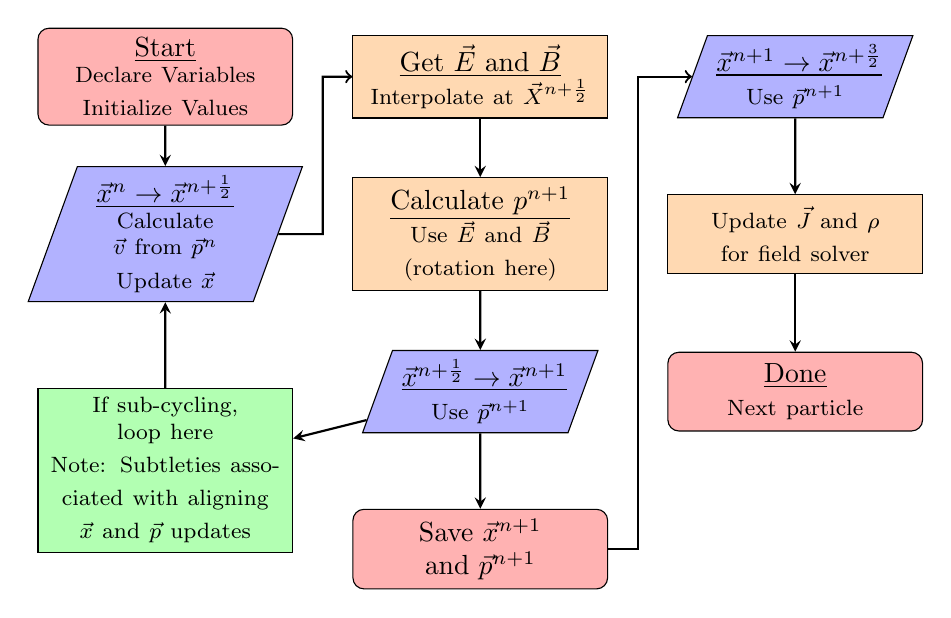
\begin{tikzpicture}[node distance=2cm]

\node (start) [startstop] {\underline{Start}\\{\footnotesize Declare Variables\\Initialize Values}};

\node(pos1)[io, below of=start]{\underline{$\vec{x}^n \rightarrow \vec{x}^{n+\frac{1}{2}}$}\\{\footnotesize Calculate $\vec{v}$ from $\vec{p}^n$\\Update $\vec{x}$}}; 

\draw[arrow](start) -- (pos1);

\node(EB)[process, right of=start, xshift=2cm]{\underline{Get $\vec{E}$ and $\vec{B}$}\\{\footnotesize Interpolate at $\vec{X}^{n+\frac{1}{2}}$}};

\draw[thick,->] (pos1) -- +(2,0) |- (EB);

\node(pn1)[process, below of=EB]{\underline{Calculate $p^{n+1}$}\\{\footnotesize Use $\vec{E}$ and $\vec{B}$ (rotation here)}};

\draw[arrow](EB) -- (pn1);

\node(pos2)[io, below of=pn1]{\underline{$\vec{x}^{n+\frac{1}{2}} \rightarrow \vec{x}^{n+1}$}\\{\footnotesize Use $\vec{p}^{n+1}$}};

\draw[arrow](pn1) -- (pos2);

\node(save)[startstop, below of=pos2]{Save $\vec{x}^{n+1}$ and $\vec{p}^{n+1}$};

\draw[arrow](pos2) -- (save);

\node(pos3)[io, right of=EB, xshift=2cm]{\underline{$\vec{x}^{n+1} \rightarrow \vec{x}^{n+\frac{3}{2}}$}\\{\footnotesize Use $\vec{p}^{n+1}$}};

\draw[thick,->] (save) -- +(2,0) |- (pos3);

\node(cur)[process, below of=pos3]{{\footnotesize Update $\vec{J}$ and $\rho$ for field solver}};

\draw[arrow](pos3) -- (cur);

\node(end)[startstop, below of=cur]{\underline{Done}\\{\footnotesize Next particle}};

\draw[arrow](cur) -- (end);

\node(sub)[decision, left of =pos2, xshift=-2cm, yshift=-1cm]{{\footnotesize If sub-cycling, loop here\\Note: Subtleties associated with aligning $\vec{x}$ and $\vec{p}$ updates}};

\draw[arrow](pos2) -- (sub);
\draw[arrow](sub) -- (pos1);

\end{tikzpicture}
\label{fig:boris}
\end{figure}

Our pusher follows the implementation in EPOCH \cite{epoch}, but with some modifications.  We use our own linear interpolation method (for simplicity), and omit the steps necessary for the field solver, which we did not implement.  We have different logic for finding the field points nearest a particle, and recursive logic to find the finest grid cell a particle is in.  In addition, we have a particle list for each base cell, and implemented logic to pass particles between lists (this makes the load balancing easier).

\subsection{Particle Lists}

\subsection{Grid Trees}

\subsection{Grid Refinement}



\section{Parallelization}

\subsection{List Passer}

\subsection{Cell Passer}

\subsection{Load Balancer}


\section{Theoretical Performance}

\section{Performance Results}

\section{Discussion}

\section{Conclusions}
























{\def\section*#1{}
\begin{thebibliography}{1}
%\footnotesize
\setlength{\itemsep}{0pt}
\bibitem{epoch}The EPOCH code was developed as part of the UK EPSRC funded projects EP/G054940/1
\bibitem{bird}Birdsall, C.K. and Langdon, A.B.  (1985). \textit{Plasma Physics via Computer Simulation}. McGraw-Hill.
%\bibitem{three}Po Kin Leung et al. 2011 Astrophysical Journal, 737 21.
%\bibitem{four}Feryal Özel et al. 2000 Astrophysical Journal, 541 234.
%\bibitem{rotation}Arefiev, Alexey V., et al. ``Temporal resolution criterion for correctly simulating relativistic electron motion in a high-intensity laser field."  Phys. Plasmas 22, 013103 (2015)

\end{thebibliography}
}




\end{document}